\begin{enumerate}[label=\thesubsection.\arabic*.,ref=\thesubsection.\theenumi]
\numberwithin{equation}{enumi}
\item
Consider the quadrature-oscillator circuit given Fig. \ref{fig:es17btech11009_fig1} without the limiter. Let the resistance $R_{f}$ be equal to $\frac{2R}{1 + \Delta}$ where $\Delta \ll 1$. Show that the poles of the characteristic equation are in the right-half s plane and given by 
s $\approx \frac{1}{CR}(\frac{\Delta}{4}\pm j)$

\renewcommand{\thefigure}{\theenumi.\arabic{figure}}
\begin{figure}[!ht]
	\begin{center}
		\resizebox{\columnwidth}{!}{\input{./figs/es17btech11009/es17btech11009_fig1.tex}}
	\end{center}
\caption{}
\label{fig:es17btech11009_fig1}
\end{figure}
\item
And the Equivalent circuit at the input of op-amp 2 is given in Fig \ref{fig:es17btech11009_fig2}
\renewcommand{\thefigure}{\theenumi.\arabic{figure}}
\begin{figure}[!ht]
	\begin{center}
		\resizebox{\columnwidth}{!}{\begin{circuitikz}
\ctikzset{bipoles/length=1cm}

 
\draw (0,0) to node[ground]{}(0,0) --(0,0.15) to[isource, l=$\frac{v_{o_1}}{2R}$] (0,3);
\draw (0,3) --(2,3) to[R=$2R$,*-*] (2,0) to node[ground]{}(2,0);
\draw (2,3) -- (4,3) to[C=$C$,*-*](4,0) to node[ground]{}(4,0) ;
\draw (4,3) --(6,3) to [R=$-R_{f}$,*-*](6,0) to node[ground]{}(6,0);
\draw (6,3) --(7,3)to node[right]{$v= \frac{v_{o_2}}{2}$}(7,3);
\end{circuitikz}

}
	\end{center}
\caption{}
\label{fig:es17btech11009_fig2}
\end{figure}

\item 
\solution

The Quadrature oscillator is based on the second integrator.

As an active filter, the loop is damped to locate the poles in the left half of the s-plane. In the quadrature oscillator, the op amp 1 is connected as an inverting miller integrator with a limiter in the feedback for controlling the amplitude. The op amp 2 is connected as a non-inverting integrator.

Draw the circuit without the limiter shown in Fig \ref{fig:es17btech11009_fig3}
\renewcommand{\thefigure}{\theenumi.\arabic{figure}}
\begin{figure}[!ht]
	\begin{center}
		\resizebox{\columnwidth}{!}{\begin{circuitikz}
\ctikzset{bipoles/length=1cm}
 
\draw (0, 0) node[op amp] (opamp) {\texttt{2}};
\draw (opamp.-) --(-1,0.35)-- (-1,1.25) to[R=$2R$,*-*] (1,1.25) -- (1,0) -- (1,-1.25) to  [vR=$R_{f}$,*-*] (-1,-1.25) -- (-1,-0.35) to (opamp.+);
\draw (-1,-1.25) to[C=$C$,*-*] (-1, -3) to node[ground]{} (-1,-3);
\draw (opamp.out) --(1,0)  --(2,0) to node[right]{$v_{o_2}$}(2,0) ;
\draw (-1,0.35) to [R=$2R$,*-*](-3.5,0.35) to node[ground]{} (-3.5,0.35);
\draw (-1,-1.25) to [R=$2R$,*-*](-4,-1.25) to node[left]{$v_{o_1}$}(-4,-1.25);
\draw node at (-1.3,0) {$\frac{v_{o_2}}{2}$};
\end{circuitikz}

}
	\end{center}
\caption{}
\label{fig:es17btech11009_fig3}
\end{figure}
\item
Draw the equivalent control system representation for the circuit in Fig. \ref{fig:es17btech11009_fig3} which is given in \ref{fig:es17btech11009_block}

\renewcommand{\thefigure}{\theenumi.\arabic{figure}}
\begin{figure}[!ht]
	\begin{center}
		\resizebox{\columnwidth}{!}{\input{./figs/es17btech11009/es17btech11009_2.tex}}
	\end{center}
\caption{Simplified equivalent block diagram}
\label{fig:es17btech11009_block}
\end{figure}

\item
From \ref{fig:es17btech11009_fig3}.

Use voltage division principle to write the expression of the fraction of its input voltage.
\begin{align}
v_{+}&= v_{-}=\brak{\frac{v_{o_2}}{2R + 2R}}\brak{2R} = \frac{v_{o_2}}{2}
\end{align}
\item
Apply KCL at the non- inverting terminal of the op amp in Fig \ref{fig:es17btech11009_fig3}
\begin{align}
\frac{\frac{v_{0_2}}{2} - v_{o_1}}{2R} + \frac{\frac{v_{0_2}}{2}}{\frac{1}{sC}} + \frac{\frac{v_{0_2}}{2} - v_{o_2}}{R_{f}} =0
\end{align}
\begin{align}
\frac{v_{o_2} - 2v_{o_1}}{4R} + sC\frac{v_{o_2}}{2} + \frac{v_{o_2} - 2v_{o_2}}{2R_{f}} = 0
\end{align}
\begin{align}
\frac{v_{o_2} - 2v_{o_1}}{4R} + sCv_{o_2} -  \frac{v_{o_2}}{R_{f}} = 0
\end{align}
\item
Substitute $R_{f} = \frac{2R}{1 + \Delta}$ and find the feedback factor H
\begin{align}
\frac{v_{o_2} - 2v_{o_1}}{4R} + sCv_{o_2} -  \frac{v_{o_2}}{2R}\brak{1 + \Delta} = 0
\end{align}
\begin{align}
v_{o_2}\brak{\frac{1}{2R} + sC - \frac{1+ \Delta}{2R}}&= \frac{v_{o_1}}{R} 
\end{align}
\begin{align}
v_{o_2}\brak{1 + 2sRC -1 - \Delta}&= 2v_{o_1}
\end{align}
Simplifying further,
\begin{align}
    \frac{v_{o_2}}{v_{o_1}}&= \frac{1}{sRC - \frac{\Delta}{2}}
\end{align}
\begin{align}
    H &=\frac{v_{o_2}}{v_{o_1}}= \frac{1}{sRC - \frac{\Delta}{2}}
    \label{eq:es17btech11009_H}
\end{align}

\item
Find the open loop gain

When we consider the circuit without the limiter and break the loop at X,
The expression for open loop gain is 
\begin{align}
    G = \frac{v_{o_2}}{v_x} = -\frac{1}{sCR}
    \label{eq:es17btech11009_G}
\end{align}
The transfer function of the equivalent positive feedback circuit in Fig. \ref{fig:es17btech11009_fig3} is  
\begin{align}
T &= \frac{G}{1-GH}
\label{eq:es17btech11009_TF}
\end{align}
Therefore, loop gain is given by 
\begin{align}
L &= GH
\end{align}
From \eqref{eq:es17btech11009_G} and \eqref{eq:es17btech11009_H}
\begin{align}
L\brak{s}&= \frac{-1}{sCR}\frac{1}{sCR - \frac{\Delta}{2}}
\end{align}
\begin{align}
L\brak{s}&= \frac{1}{-s^2C^2R^2 + \frac{sCR\Delta}{2}}
\end{align}
Consider the characteristic equation of the transfer function \eqref{eq:es17btech11009_TF},
\begin{align}
    1 - L\brak{s} = 0
\end{align}
\begin{align}
    L\brak{s} = 1
\end{align}
\begin{align}
    -s^2C^2R^2 + \frac{sCR\Delta}{2} = 1
\end{align}
\begin{align}
    \brak{C^2R^2}s^2 + \brak{-\frac{CR\Delta}{2}}s + 1 = 0
\end{align}
\item
Write the expression for roots of a general quadratic equation
\begin{align}
    s_{p} = \frac{-b \pm \sqrt{b^2 - 4ac}}{2a}
    \label{eq:es17btech11009_quad}
\end{align}
 Substitute $a=C^2R^2$, $b=-\frac{CR\Delta}{2}$, $c=1$ in \eqref{eq:es17btech11009_quad},
 \begin{align}
     s_{p} = \frac{-\brak{-\frac{CR\Delta}{2}} \pm \sqrt{\brak{-\frac{CR\Delta}{2}}^2 - 4\brak{C^2R^2}\brak{1}}}{2C^2R^2}
 \end{align}
 \begin{align}
      = \frac{RC\brak{\frac{\Delta}{2} \pm \sqrt{\brak{\frac{\Delta}{2}}^2 -4}}}{2C^2R^2}
 \end{align}
 \begin{align}
      = \frac{\frac{\Delta}{2} \pm \sqrt{\brak{\frac{\Delta}{2}}^2-4}}{2RC}
 \end{align}
 \begin{align}
      = \frac{\frac{\Delta}{2} \pm 2j\sqrt{1 - \brak{\frac{\Delta}{4}}^2}}{2RC}
 \end{align}
 As $\Delta \ll 1$, 
 \begin{align}
     \brak{1-\brak{\frac{\Delta}{4}}^2}^\frac{1}{2} = 1 - \frac{1}{2}\brak{\frac{\Delta}{4}}^2
 \end{align}
 \begin{align}
 s_{p} = \frac{\frac{\Delta}{2} \pm 2j\brak{1 - \frac{1}{2}\brak{\frac{\Delta}{4}}^2}}{2RC}
 \end{align}
 \begin{align}
  s_{p}= \frac{\frac{\Delta}{2} \pm j\brak{2 - \brak{\frac{\Delta}{4}}^2}}{2RC}
  \label{eq:es17btech11009_eqn}
 \end{align}
 From \eqref{eq:es17btech11009_eqn},
 \begin{align}
     Re\brak{s_{p}} \textgreater 0
 \end{align}
 Hence, the poles of the characteristic equation are in the right half of the s plane.
 
 As $\Delta \ll 1$, higher order terms are neglected.
 \begin{align}
     s_{p} = \frac{\frac{\Delta}{2} \pm 2j}{2RC}
 \end{align}
 \begin{align}
     s_{p} = \frac{\frac{\Delta}{4} \pm j}{RC}
 \end{align}
 
\item 
Find the frequency for arbitrary R,C values as given in Table \ref{table:es17btech11009_Table1}
\begin{table}[!ht]
\centering
\input{./tables/es17btech11009/es17btech11009_table1.tex}
\caption{}
\label{table:es17btech11009_Table1}
\end{table}

The loop will oscillate at frequency $\omega_{o}$, given by
\begin{align}
    \omega_{o} = \frac{1}{RC}
\end{align}
From Table \ref{table:es17btech11009_Table1},
\begin{align}
    \omega_{o} = 1rad/s
\end{align}
\begin{align}
    f = \frac{\omega_{o}}{2\pi} = 0.159 Hz
\end{align}
Substituting \eqref{eq:es17btech11009_G} and \eqref{eq:es17btech11009_H} in \eqref{eq:es17btech11009_TF},
\begin{align}
    T = \frac{-SCR + \frac{\Delta}{2}}{s^2C^2R^2 - \frac{sCR\Delta}{2} + 1}
\end{align}
Taking values from Table \ref{table:es17btech11009_Table1},
\begin{align}
    T = \frac{-s + 0.05}{s^2 - 0.05s +1}
\end{align}
The following code plots the oscillating response of the system as given in Fig \ref{fig:es17btech11009_1_1}
\begin{lstlisting}
codes/es17btech11009/es17btech11009_1_1.py
\end{lstlisting}
\begin{figure}[!ht]
\centering
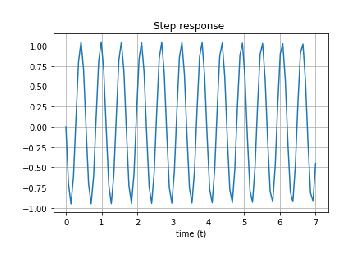
\includegraphics[width=\columnwidth]{./figs/es17btech11009/es17btech11009_1_1.eps}
\caption{}
\label{fig:es17btech11009_1_1}
\end{figure}
\item
Simulate the circuit Fig \ref{fig:es17btech11009_fig3} using spice simulators and plot the generated output using python script.

Find the netlist for the simulated circuit here:
\begin{lstlisting}
spice/es17btech11009.net
\end{lstlisting}
Python code used for generating the output:
\begin{lstlisting}
spice/es17btech11009_spice.py
\end{lstlisting}
\begin{figure}[!ht]
\centering
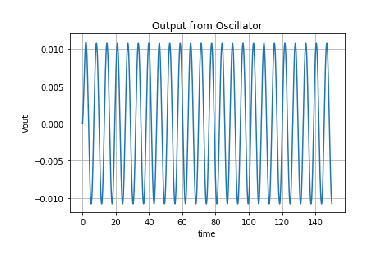
\includegraphics[width=\columnwidth]{./figs/es17btech11009/es17btech11009_spice.eps}
\caption{}
\label{fig:es17btech11009_spice}
\end{figure}
From the Fig \ref{fig:es17btech11009_spice},
Time period of oscillation 
\begin{align}
    T = 6.28 s
\end{align}
\begin{align}
    f = \frac{1}{T} = 0.159
\end{align}
\begin{align}
    \omega_{o} = 2\pi f = 0.998
\end{align}
Hence the frequency calculated from the formulae and the plot are approximately same.
\end{enumerate}
